\documentclass{JNUexp}
\courseName{计算机图形学}
\expName{实验 3 线段的裁剪与参数化曲线}
\expDate{2017.11.16}
\className{计科1404}
\studentName{阎覃}
\studentId{1030414414}

\graphicspath{ {images/} }

\usepackage[hidelinks]{hyperref}
\usepackage{amsmath}
\begin{document} 

\section{实验内容}
\begin{itemize}
    \item 实现编码算法或liang-barsky算法 
    \item 绘制一条Bezier曲线及其控制多边形
\end{itemize}

\section{实验步骤及运行情况}
%%%%%%%%%%%%%%%%%%%%%%%%%%%%%%%%%%%%%%%%%%%%%%%%%%%%%%%%%
%   1 实现编码算法或liang-barsky算法 
%%%%%%%%%%%%%%%%%%%%%%%%%%%%%%%%%%%%%%%%%%%%%%%%%%%%%%%%%
\begin{problem}
    实现编码算法或liang-barsky算法  
\end{problem}
\begin{answer}
    \lstinputlisting[language={[11]C++},title=Entities/LineClipLB2D.cpp]{../src/Entities/LineClipLB2D.cpp}
    本程序参考书上代码P123。
\end{answer}
\begin{image}
    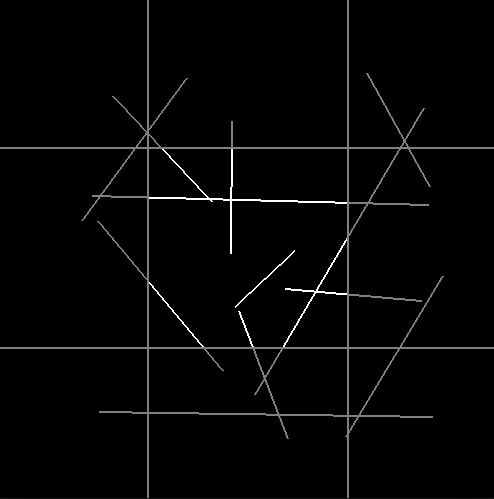
\includegraphics[width=0.7\textwidth]{1}
\end{image}
%%%%%%%%%%%%%%%%%%%%%%%%%%%%%%%%%%%%%%%%%%%%%%%%%%%%%%%%%
%   2 绘制一条Bezier曲线及其控制多边形
%%%%%%%%%%%%%%%%%%%%%%%%%%%%%%%%%%%%%%%%%%%%%%%%%%%%%%%%%
\begin{problem}
    绘制一条Bezier曲线及其控制多边形  
\end{problem}
\begin{answer}
    n次Bezier曲线的数学表达式如下
    \begin{align}
        Q(t) &= \sum^n_{i=0}{P_iB_{i,n}(t)},t\in [0,1] \\
        B_{i,n}(t) &= \frac{n!}{i!(n-i)!}t^i(1-t)^{n-i},i=0,1,\dots,n
    \end{align}
    
    de Casteljau算法用下面的迭代公式计算型值点$Q(t)$
    \begin{equation*}
        P^r_i = \left\{
        \begin{aligned}
            & P_i  && r=0 \\ 
            & (1-t)P_i^{r-1}+tP_{i+1}^{r-1}  && r=1,2,\dots,n
        \end{aligned}
        \right.
        i=0,1,\dots,n-r
    \end{equation*}

    可以用数学归纳法证明,型值点$Q(t)$就是$P_0^n$

    \lstinputlisting[language={[11]C++},title=Entities/BezierCas2D.cpp]{../src/Entities/BezierCas2D.cpp}
\end{answer}
\begin{image}
    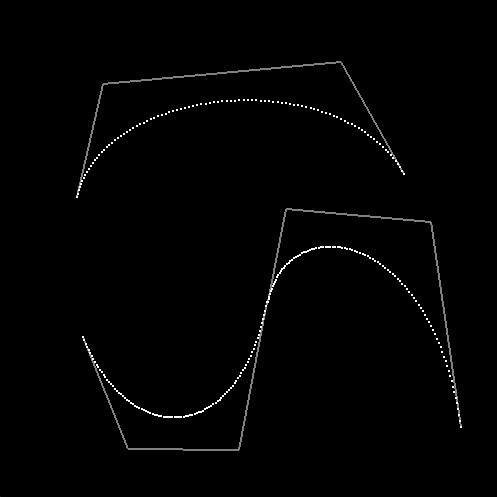
\includegraphics[width=0.7\textwidth]{2}
\end{image}
\newpage
\section{实验体会}
线段裁剪算法有很多,本次试验实现的是Liang-Barsky算法。程序中设定了一个裁剪窗口,在窗口外的线用
灰色表示,窗口内被裁剪的线段用白色表示。本程序可以实现绘制n阶Bezier曲线,在程序中修改n的值即可。
控制多边形用灰色表示。

\vfill

实验报告采用 \LaTeX 排版,完整代码托管至GitHub:\\
\url{https://github.com/Ethan-yt/JNU-CG-exp}

\end{document}